% Section 5 -- Extraction conventions. The umbrella result: template mode, read position, tensor identity.
% Scoping rule: the templating claim is made for harmful-content probing ONLY (Section 5.4).
\section{Extraction Conventions}
\label{sec:extraction}

A probe is usually described by its training set, its layer, and its threshold. Those three choices are what papers
report. This section is about three choices that papers do not report---which text the activation is read from, which
token position it is read at, and which tensor at that layer is read---and shows that on these tasks they dominate the
ones that are reported.

We use \emph{extraction convention} as the umbrella term for the three. Figure~\ref{fig:extraction} previews the two
that are repairable, on every model.

% Plain figure*, NOT the class's \Figure macro: \Figure sets \xfigwd to the graphic's width, which sends
% \@makecaption down a branch that typesets the caption in a non-wrapping tabular. See the \xfigwd note in
% main.tex. Captions here are long, so they must wrap.
\begin{figure*}[!t]
\centering
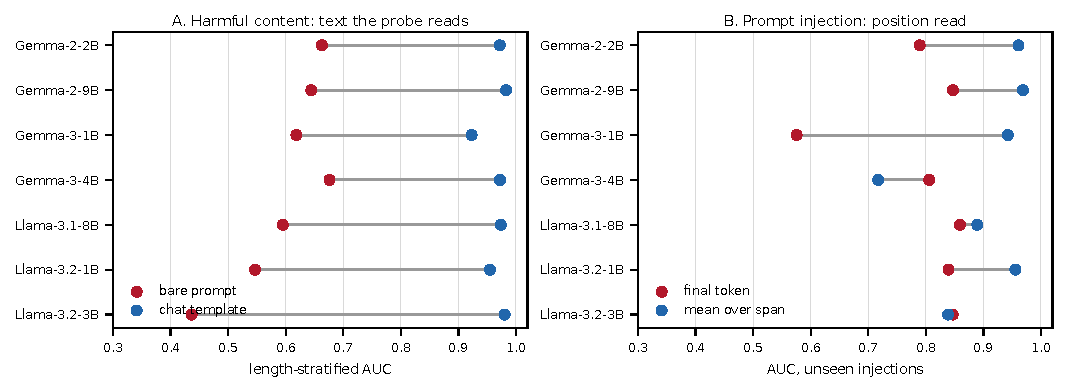
\includegraphics[width=\textwidth]{figures/fig_extraction}
\caption{The extraction convention, not the probe, decides the outcome. Each line joins one model's score under two
reads of the same activation, with everything else held fixed. \textbf{A}: harmful-content probes read at the final
token of the bare prompt versus of the prompt in the model's own chat template, for probes fitted with on-topic
negatives; length-stratified AUC rises by $+0.296$ to $+0.544$, to $0.923$--$0.983$, on all seven models. The probes
as shipped, fitted on off-topic negatives, do not share the gain: three of them regress under the templated read
(Table~\ref{tab:extraction_convention}). \textbf{B}: prompt-injection probes read at the final token versus averaged
over the tool-response span, on the grouped split in which no injection string in the test half was seen in training;
the four models on which the mean read clears the pre-registered $0.90$ pass threshold move from $0.58$--$0.85$ to
$0.94$--$0.97$, three never reach the pass band, and Gemma-3-4B is worse at the point estimate. Neither change touches
the probe or its training data.}
\label{fig:extraction}
\end{figure*}

\subsection{Template mode: reading the prompt as the model will see it}
\label{sec:template}

An instruction-tuned model never sees a bare user prompt in deployment. It sees that prompt wrapped in a chat
template that marks the turn boundary and cues the model that a response is expected. A probe can be read either way,
and the choice is rarely stated.

Table~\ref{tab:extraction_convention} holds everything else fixed---the same $300$ harmful prompts, the same $350$
benign prompts, the same layer, the same tensor, the same threshold rule---and varies only whether the final-token
activation is taken from the bare prompt or from the templated one. Three probes are shown per model: the shipped
probe as distributed, a probe trained on on-topic benign twins, and a probe trained on the off-topic negatives the
shipped probes were originally fitted with.

% GENERATED by paper/tools/gen_tables.py -- do not edit by hand.
% sources: results/gates/extraction_convention.json
\begin{table*}[!t]
\caption{Extraction convention: the same probes, prompts, layers and feature, read at the final token of the
bare prompt versus of the prompt in the model's own chat template. AUC$^{*}$ is length-stratified. JBB FPR@m is
the JailbreakBench-benign false-positive rate at the threshold whose XSTest FPR matches the shipped probe's, so
the FPR columns are comparable across probes rather than reflecting a threshold shift. Training negatives:
on-topic twins versus the off-topic set the shipped probes were trained on.}
\label{tab:extraction_convention}
\centering
\setlength{\tabcolsep}{3.5pt}
\footnotesize
\begin{tabular}{llccccccc}
\toprule
& Negatives & AUC$^{*}$ raw & AUC$^{*}$ tmpl & $\Delta$ & AUC vs JBB raw & AUC vs JBB tmpl & FPR@m raw & FPR@m tmpl \\
\midrule
Gemma-2-2B & shipped & 0.754 & 0.875 & +0.121 & 0.485 & 0.717 & 0.80 & 0.04 \\
 & on-topic & 0.663 & 0.972 & +0.309 & 0.825 & 0.909 & 0.00 & 0.00 \\
 & off-topic & 0.828 & 0.979 & +0.152 & 0.690 & 0.910 & 0.67 & 0.00 \\
\addlinespace
Gemma-2-9B & shipped & 0.841 & 0.982 & +0.142 & 0.640 & 0.937 & 0.76 & 0.05 \\
 & on-topic & 0.645 & 0.983 & +0.338 & 0.800 & 0.906 & 0.03 & 0.07 \\
 & off-topic & 0.827 & 0.982 & +0.155 & 0.824 & 0.888 & 0.43 & 0.10 \\
\addlinespace
Gemma-3-1B & shipped & 0.689 & 0.706 & +0.017 & 0.539 & 0.719 & 0.89 & 0.00 \\
 & on-topic & 0.619 & 0.923 & +0.304 & 0.789 & 0.865 & 0.05 & 0.01 \\
 & off-topic & 0.637 & 0.935 & +0.298 & 0.600 & 0.866 & 0.68 & 0.04 \\
\addlinespace
Gemma-3-4B & shipped & 0.703 & 0.687 & -0.016 & 0.578 & 0.613 & 0.29 & 0.02 \\
 & on-topic & 0.676 & 0.972 & +0.296 & 0.603 & 0.868 & 0.22 & 0.00 \\
 & off-topic & 0.692 & 0.977 & +0.285 & 0.592 & 0.862 & 0.26 & 0.00 \\
\addlinespace
Llama-3.1-8B & shipped & 0.770 & 0.387 & -0.383 & 0.456 & 0.454 & 0.99 & 0.00 \\
 & on-topic & 0.595 & 0.974 & +0.379 & 0.769 & 0.933 & 0.00 & 0.02 \\
 & off-topic & 0.767 & 0.977 & +0.209 & 0.588 & 0.936 & 0.96 & 0.05 \\
\addlinespace
Llama-3.2-1B & shipped & 0.773 & 0.753 & -0.019 & 0.672 & 0.878 & 0.91 & 0.70 \\
 & on-topic & 0.547 & 0.955 & +0.408 & 0.770 & 0.878 & 0.00 & 0.75 \\
 & off-topic & 0.780 & 0.949 & +0.169 & 0.754 & 0.864 & 0.57 & 0.99 \\
\addlinespace
Llama-3.2-3B & shipped & 0.757 & 0.959 & +0.202 & 0.531 & 0.947 & 0.99 & 0.02 \\
 & on-topic & 0.437 & 0.980 & +0.544 & 0.702 & 0.928 & 0.00 & 0.05 \\
 & off-topic & 0.778 & 0.981 & +0.204 & 0.666 & 0.923 & 0.97 & 0.24 \\
\addlinespace
\bottomrule
\end{tabular}

\footnotesize Template effect (on-topic probe, AUC$^{*}$, templated $-$ raw): min $+0.296$, max $+0.544$, mean $+0.368$; positive on all 7 models. On-topic-twins effect (templated, AUC vs JBB, on-topic $-$ off-topic): min $-0.003$, max $+0.018$, mean $+0.005$.
\end{table*}

The templated read is better on every model. For the probe trained on on-topic twins, length-stratified AUC rises by
between $+0.296$ and $+0.544$, with a mean of $+0.368$, and there is no model on which it falls. Every one of those
seven differences excludes zero under a paired case bootstrap, the weakest lower bound being $+0.228$ on Gemma-3-1B
(Appendix~\ref{app:ci}, panel A), so ``positive on all seven models'' is a statement about intervals and not only
about point estimates. The effect is largest
precisely where the bare read was worst: on Llama-3.2-3B the same direction moves from $0.437$ to $0.980$.

The claim is about probes fitted with on-topic negatives, and the scope is not decorative. The shipped probes, whose
negatives are the off-topic set they were originally fitted with, do not share it: templating helps four of them but
costs Gemma-3-4B $-0.016$, Llama-3.2-1B $-0.019$ and Llama-3.1-8B $-0.383$, the last moving from $\aucstar{} = 0.770$
to $0.387$. Templating is therefore not a universal improvement to any probe one happens to hold. What
Table~\ref{tab:extraction_convention} supports is narrower: with the release recipe's training negatives replaced by
on-topic twins and everything else held fixed, reading through the chat template improves every model.

The false-positive picture moves with it, and this is the part that matters for deployment. Reported against on-topic
benign prompts at an operating point matched to each model's shipped-probe XSTest false-positive rate, the templated
read reduces the JailbreakBench false-positive rate to between $0.00$ and $0.07$ for six of seven models, against
$0.30$--$0.99$ for the shipped bare-read probes. Threshold-free, AUC against on-topic benign prompts rises from
$0.46$--$0.67$ to $0.87$--$0.93$. Table~\ref{tab:af_verdict} evaluates this against the pre-registered criteria: six
of seven models pass all three. The seventh, Llama-3.2-1B, is not evaluable on the false-positive criterion rather
than failing it, because that criterion is defined relative to the shipped probe's XSTest false-positive rate and for
this model in templated mode that rate is $0.76$, which anchors the matched operating point at a value where the
comparison is mechanically degenerate. It passes the other two criteria.

% GENERATED by paper/tools/gen_tables.py -- do not edit by hand.
% sources: results/gates/b1/*.json
\begin{table}[!t]
\caption{AF criteria on the chat-templated read (pre-registered thresholds: length-stratified AUC $\geq 0.80$;
JailbreakBench FPR at the matched-XSTest operating point $\leq 0.30$; AUC vs JailbreakBench $\geq 0.70$).}
\label{tab:af_verdict}
\centering
\setlength{\tabcolsep}{3.5pt}
\footnotesize
\begin{tabular}{lcccc}
\toprule
Model & AUC$^{*}$ & JBB FPR@m & AUC vs JBB & Verdict \\
\midrule
Gemma-2-2B & 0.972 & 0.00 & 0.909 & pass \\
Gemma-2-9B & 0.983 & 0.07 & 0.906 & pass \\
Gemma-3-1B & 0.923 & 0.01 & 0.865 & pass \\
Gemma-3-4B & 0.972 & 0.00 & 0.868 & pass \\
Llama-3.1-8B & 0.974 & 0.02 & 0.933 & pass \\
Llama-3.2-1B & 0.955 & 0.75$^{\dagger}$ & 0.878 & n/e \\
Llama-3.2-3B & 0.980 & 0.05 & 0.928 & pass \\
\bottomrule
\end{tabular}

\footnotesize $^{\dagger}$Not evaluable: the matched operating point is anchored at this model's shipped-probe
XSTest FPR of 0.76 in templated mode, so the comparison is mechanically degenerate. Criteria 1 and 3 pass.
\end{table}

Table~\ref{tab:af_lexical} confirms the result is not a lexical artifact. The strongest cheap text baseline we could
construct reaches $\aucstar{} = 0.710$ overall and $0.637$ against on-topic benign prompts; the templated probe beats
it by between $+0.213$ and $+0.272$. The same table carries the warning that motivates the length control: the
strongest \emph{unstratified} feature is character length, at $0.903$.

% GENERATED by paper/tools/gen_tables.py -- do not edit by hand.
% sources: results/gates/lexical_baselines.json
\begin{table}[!t]
\caption{Lexical baselines for harmful-content detection: cheap text features scored on the same
$300$ HarmBench prompts against the same benign sets, with no model and no activations. The
length-stratified columns are the ones comparable with probe numbers.}
\label{tab:af_lexical}
\centering
\setlength{\tabcolsep}{3.5pt}
\footnotesize
\begin{tabular}{lcccc}
\toprule
Feature & AUC & AUC$^{*}$ & vs JBB & vs JBB$^{*}$ \\
\midrule
imperative stem & 0.683 & 0.710 & 0.362 & 0.517 \\
``how to'' pattern & 0.556 & 0.606 & 0.575 & 0.607 \\
harm lexicon (count) & 0.667 & 0.590 & 0.664 & 0.595 \\
harm lexicon (any) & 0.654 & 0.584 & 0.647 & 0.589 \\
character length & 0.903 & 0.578 & 0.768 & 0.552 \\
harm lexicon $+$ ``how to'' & 0.681 & 0.632 & 0.686 & 0.637 \\
\bottomrule
\end{tabular}

\footnotesize Strongest length-stratified baseline: imperative stem at $0.710$. Note that the strongest \emph{unstratified} feature is character
length itself, at $0.903$, which is why every AUC in this
paper is reported length-stratified.
\end{table}

\subsection{Read position: where in a long input the signal lives}
\label{sec:read}

Harmful-content probing reads a short prompt, so the final token is a reasonable place to look. Agent-injection
detection reads a scaffold in which the injected instruction sits inside a tool response, and there the final token
is the wrong place by construction: across the $1{,}054$ cases the injection ends at a median $85\,\%$ of the
tool-response span and never at its end, so a final-token read is separated from the signal by the tail of the tool
output and the turn boundary.

We compare four reads at the same layer. \emph{final} is the final prompt token. \emph{mean} averages the activation
over the tool-response span. \emph{maxpos} takes the maximum projection over positions in that span. \emph{oracle} is
read at the token where the injected instruction ends; it uses label knowledge, is never deployable, and is included
as a diagnostic upper bound---if even the oracle is weak, the limitation is in the representation rather than in the
choice of position. For benign cases, which have no injection, the oracle position is drawn from the empirical
distribution of injection-end positions in the training half, so that read position itself carries no label
information.

% GENERATED by paper/tools/gen_tables.py -- do not edit by hand.
% sources: results/gates/b2/*.json, results/gates/b2_grouped/*.json, results/gates/validity_checks.json
\begin{table*}[!t]
\caption{Prompt-injection detection by read position, on the held-out half of real InjecAgent. Left block:
the pre-registered per-case split, in which all $62$ injection strings appear in both halves. Right block: the
grouped split, in which whole injection strings are assigned to one side, so no injection in the test half was
seen in training. \emph{mean} pools over the tool-response span; mean\textsubscript{all} pools over every
prompt token and is the whole-input baseline of prior work. \emph{oracle} is handed the injection's end
position and is a diagnostic bound, never deployable. The grouped test half holds $493$ injected cases against only $59$ benign ones, drawn from $62$ distinct injection strings: grouping removes the leakage, it does not create a large sample of injection types, and the intervals in Appendix~\ref{app:ci} are correspondingly wide. Quote these AUCs with their intervals.}
\label{tab:aag_designs}
\centering
\setlength{\tabcolsep}{3.0pt}
\footnotesize
\begin{tabular}{lccccccccccc}
\toprule
& \multicolumn{5}{c}{Injections seen in training} & \multicolumn{5}{c}{Injections unseen} & \\
\cmidrule(lr){2-6}\cmidrule(lr){7-11}
Model & final & mean & mean\textsubscript{all} & maxpos & oracle & final & mean & mean\textsubscript{all} & maxpos & oracle & oracle$-$best \\
\midrule
Gemma-2-2B & 0.774 & 0.964 & 0.936 & 0.951 & 0.992 & 0.789 & 0.961 & 0.937 & 0.944 & 0.978 & +0.028 \\
Gemma-2-9B & 0.849 & 0.970 & 0.921 & 0.975 & 0.997 & 0.847 & 0.969 & 0.927 & 0.963 & 0.990 & +0.022 \\
Gemma-3-1B & 0.546 & 0.845 & 0.782 & 0.824 & 0.796 & 0.576 & 0.943 & 0.849 & 0.919 & 0.865 & -0.049 \\
Gemma-3-4B & 0.796 & 0.758 & 0.783 & 0.635 & 0.774 & 0.806 & 0.717 & 0.762 & 0.616 & 0.751 & -0.022 \\
Llama-3.1-8B & 0.853 & 0.858 & 0.784 & 0.822 & 0.987 & 0.859 & 0.889 & 0.815 & 0.825 & 0.963 & +0.129 \\
Llama-3.2-1B & 0.828 & 0.949 & 0.882 & 0.931 & 0.994 & 0.839 & 0.956 & 0.906 & 0.931 & 0.982 & +0.045 \\
Llama-3.2-3B & 0.840 & 0.818 & 0.741 & 0.747 & 0.987 & 0.847 & 0.839 & 0.763 & 0.770 & 0.961 & +0.148 \\
\bottomrule
\end{tabular}

\footnotesize Mean AUC change when injection strings are unseen: final $-0.011$, mean $-0.016$, maxpos $-0.012$, oracle $+0.005$. The result is generalisation to unseen injections, not recognition of memorised strings. Span localisation (mean $-$ mean\textsubscript{all}, unseen split): $-0.044$ to $+0.093$; positive on 6 of 7 models (intervals in Appendix~\ref{app:ci}).
\end{table*}

Averaging over the tool-response span recovers most of what the final-token read misses. On the four models on which
the mean read clears the pass threshold of $0.90$ that was pre-registered before any activation was extracted
(Section~\ref{sec:prereg}), mean-over-tool-response reading reaches $0.94$--$0.97$ against $0.58$--$0.85$ for the final-token
read trained on identical data; on those four the paired difference excludes zero, with a smallest lower bound of
$+0.067$ (Appendix~\ref{app:ci}, panel B). On the other three it does not: the interval crosses zero on Llama-3.1-8B
($+0.030$, $[-0.022, +0.082]$), on Llama-3.2-3B ($-0.008$, $[-0.062, +0.047]$) and on Gemma-3-4B, where the mean read
is worse at the point estimate ($-0.089$, $[-0.198, +0.026]$). Both figures are quoted from the grouped split, and the
full seven-model picture is in Table~\ref{tab:aag_designs} rather than summarised away.

Localisation, not pooling as such, is what the span read adds. Prior work already compares mean pooling with
last-token reads (Section~\ref{sec:related}), so Table~\ref{tab:aag_designs} carries the whole-prompt mean,
mean\textsubscript{all}, as the baseline that claim is defined against; the comparison was pre-registered with its
threshold before the run (Section~\ref{sec:prereg}). On the four passing models the tool-response mean exceeds the
whole-prompt mean by $+0.023$ to $+0.093$, every paired interval excluding zero, and by $+0.074$ and $+0.076$ on
Llama-3.1-8B and Llama-3.2-3B; only on Gemma-3-4B, where no read works, is the whole-prompt mean ahead ($-0.044$,
$[-0.106, +0.011]$). The honest reading cuts both ways: pooling over the whole input already clears the pass threshold
on three of the four models (Gemma-3-1B is the exception, at $0.849$), so most of the repair is pooling at all, and
localising the pool to the span where the threat sits is a measurable further gain rather than the whole effect. The remaining three models divide in a way worth stating: on
Llama-3.1-8B and Llama-3.2-3B no deployable read reaches the pass band, yet the oracle reaches $0.963$ and $0.961$, so
the signal is present and it is position-finding that fails to capture it without label knowledge; on Gemma-3-4B no
read works at all, and the oracle ($0.751$) is below that model's own final-token read, so there is nothing at the
injection position for a better-placed read to find.

The right-hand block of Table~\ref{tab:aag_designs} is the result we rest on. Because the corpus crosses only $62$
injection strings with $17$ user instructions, a case-level split leaves every test-half injection string present in
training, and any number computed on it measures recognition. Assigning whole injection strings to one side removes
that: the mean AUC change across models is between $-0.016$ and $+0.005$ for every read. The improvement is
generalisation to injections never seen, not memorisation. The corpus still contains only $62$ injection strings: the
grouped split removes the leakage, it does not create a large sample of injection types. The grouped test half holds
only $59$ benign cases, which
is why the intervals in Appendix~\ref{app:ci} are wide; the per-case split, with all $120$ benign cases in play,
agrees with it to within $0.016$ and is the corroboration rather than the headline.

The oracle reaches $0.96$--$0.99$ on five models, and the gap between it and the best deployable read is $+0.02$ to
$+0.15$ on those five and negative on two. Most of the available signal is therefore already reachable without label
knowledge, which is the useful form of the result: a deployable read captures nearly what a read placed by an oracle
does. A three-layer check around each model's fixed layer moves the oracle by at most $0.09$ and does not change the
ordering of the reads; we report it as a note and do not move the headline layer, since a layer selected on the
evaluation half would not be held out.

Refusal separation shows the probe is not redundant with model behaviour here. The models refuse only $3$--$25\,\%$ of
injection prompts and follow the injected instruction in $2$--$5\,\%$ of generations, so there is little behavioural
signal for the probe to be re-detecting---in contrast to harmful-content probing, where the shipped probe's flags
largely coincide with the model's own refusals (Table~\ref{tab:af_refusal}, Section~\ref{sec:topicharm}).

\subsection{Tensor identity: which activation the probe was actually trained on}
\label{sec:tensor}

The third convention is the least visible and the easiest to get wrong. A common way to capture activations is a
forward hook on a decoder layer taking the first element of its output. In HuggingFace Transformers that element is
the post-block residual stream. In vLLM, whose Gemma-2, Llama and Qwen-2 decoder layers return
\texttt{(mlp\_branch, residual)} because the residual addition is deferred to the next layer's fused normalisation,
the same line of code captures the MLP-branch output instead. The two are different tensors, and a probe fitted
through one and evaluated through the other is not the same probe.

The return convention itself is not a discovery of ours. It is documented in the tooling community---in project
writeups on capturing activations from vLLM \cite{nnsight2026hooks}, in a vLLM issue thread on the layer return
signature \cite{vllmissue12099}, and implicitly in the existence of dedicated inspection libraries that exist partly
to paper over it \cite{vllmlens}. What has not been quantified is the silent research consequence, and that is our
contribution here.

We encountered it by scoring an identical probe on identical prompts through two independent implementations and
finding a correlation of only $0.74$ where reimplementation noise should have given essentially $1.0$.
Table~\ref{tab:tensor_identity} resolves it: read as the MLP-branch output, the same probe reproduces the original
scores at $r = 0.9998$.

% GENERATED by paper/tools/gen_tables.py -- do not edit by hand.
% sources: results/phase2/p2_summary.json, results/phase2/p2_summary_mlp.json
\begin{table}[!t]
\caption{Tensor identity. A vLLM decoder layer returns \texttt{(mlp\_branch, residual)}, so a forward hook
taking \texttt{output[0]} captures the MLP-branch output, not the residual stream. Scoring the same probe on
the same prompts through an independent HuggingFace path identifies which tensor the shipped probes live in.}
\label{tab:tensor_identity}
\centering
\begin{tabular}{lcc}
\toprule
Feature read & Pearson $r$ & mean $|\Delta|$ \\
\midrule
post-block residual stream & 0.7423 & 0.0273 \\
MLP-branch output & 0.9998 & 0.0004 \\
\bottomrule
\end{tabular}

\footnotesize $n=6200$ prompts. The probes live in the MLP-branch space; every number in this
paper is computed there.
\end{table}

The failure mode is the dangerous kind, because nothing breaks. Training and evaluation used the same hook, so results
obtained this way remain internally valid and look entirely plausible; only their description is wrong, and a reader
has no way to tell. A reimplementation that agrees with the original to two decimal places may still be reading a
different tensor, and at $r = 0.74$ the disagreement is large enough to change conclusions while small enough to be
mistaken for numerical noise. ``Layer $\ell$ activation'' is therefore underspecified as a description of a probe.

The structural remedy is an interface that makes the captured tensor explicit rather than incidental to a hook's
position in a call stack; an RFC we co-authored proposes one for vLLM \cite{vllmrfc36998}. Every number in this paper is computed in
the MLP-branch space, which is where the probes under study live.

\subsection{Scope of the templating claim}
\label{sec:scope}

The claim in Section~\ref{sec:template} is made for harmful-content probing only.

``Templated'' is not one operation. For a short user prompt it wraps the text in a user turn, which is exactly what
the model sees at deployment; the templated read is the ecologically valid one and the bare read is the artifact. For
an agent scaffold it wraps an entire multi-turn transcript inside a single user turn, which corresponds to nothing
the model sees in use. For a policy-compliance case it wraps a model \emph{response} as though the model had received
it as input, which is stranger still.

We therefore report the other two tasks in both modes as observations and draw no hypothesis test from them.
Table~\ref{tab:aag_modes} gives the agent-scaffold comparison: templating helps the final-token read on four models
by $+0.04$ to $+0.15$, is neutral on two, and hurts one by $-0.14$, while the mean-span and oracle reads barely move.
That is a different pattern from the uniform, large improvement in Table~\ref{tab:extraction_convention}, and it is
consistent with the two operations being different rather than with a single effect of ``using the chat template''.

% GENERATED by paper/tools/gen_tables.py -- do not edit by hand.
% sources: results/gates/b2/*.json, results/gates/b2_templated/*.json
\begin{table}[!t]
\caption{Agent-scaffold read, bare versus chat-templated (raw / templated). Reported as an observation, not as
a test of the harmful-content result: wrapping an entire agent transcript in a user turn is a different
operation from templating a bare user prompt.}
\label{tab:aag_modes}
\centering
\setlength{\tabcolsep}{2.0pt}
\scriptsize
\begin{tabular}{lcccc}
\toprule
Model & final & mean & mean\textsubscript{all} & oracle \\
\midrule
Gemma-2-2B & 0.774 / 0.880 & 0.964 / 0.959 & 0.936 / 0.932 & 0.992 / 0.993 \\
Gemma-2-9B & 0.849 / 0.891 & 0.970 / 0.954 & 0.921 / 0.902 & 0.997 / 0.999 \\
Gemma-3-1B & 0.546 / 0.692 & 0.845 / 0.913 & 0.782 / 0.869 & 0.796 / 0.810 \\
Gemma-3-4B & 0.796 / 0.661 & 0.758 / 0.738 & 0.783 / 0.749 & 0.774 / 0.711 \\
Llama-3.1-8B & 0.853 / 0.849 & 0.858 / 0.848 & 0.784 / 0.775 & 0.987 / 0.994 \\
Llama-3.2-1B & 0.828 / 0.886 & 0.949 / 0.958 & 0.882 / 0.873 & 0.994 / 0.991 \\
Llama-3.2-3B & 0.840 / 0.841 & 0.818 / 0.809 & 0.741 / 0.753 & 0.987 / 0.990 \\
\bottomrule
\end{tabular}
\end{table}

The general form of the recommendation is not ``apply the chat template''. It is that the extraction convention is a
free parameter which current practice leaves unreported, that its effect on these tasks is larger than the effects
papers do report, and that a probe result is uninterpretable without it. Text form, token position, and tensor
identity should be stated as routinely as the layer index.
